\documentclass[11pt,a4paper]{article}

\usepackage[applemac]{inputenc}
\usepackage{latexsym}
\usepackage{graphicx}
\usepackage[francais]{babel}
\usepackage{amsmath,amssymb}
\usepackage{pstricks,pst-plot}
\usepackage{calc}
\usepackage{multicol}
\usepackage{fancyhdr}
\usepackage{lastpage}
\usepackage[T1]{fontenc}
\usepackage[top=3.5cm, bottom=2.5cm, left=1.5cm, right=1.5cm]{geometry}
\usepackage{stmaryrd}
\usepackage{float}
\pagestyle{plain}
\usepackage{epstopdf}
\usepackage{stmaryrd} 


\title{TP 2 \\ The stochastic multi-armed bandit}
\author{Mathurin \textsc{Massias} \and Clement \textsc{Nicolle}}
\date{\today} 

\begin{document}
\maketitle

\section{Building a MAB problem}
\hspace{-6mm} We replaced the initial parameters by :
\begin{verbatim}
Arm1=armBernoulli(0.4); %mean 0.4
Arm2=armBeta(4,12); %mean 0.25
Arm3=armExp(9); %mean 0.11
Arm4=armFinite([0.2 0.4 0.7 0.8],[0.1 0.3 0.3 0.3]); %mean 0.59

MAB={Arm1,Arm2,Arm3,Arm4};
\end{verbatim}

\section{The UCB algorithm}

\hspace{-6mm} We implemented the naive strategy in \textit{naive.m}, simply by calling \textit{UCB.m} with parameter $\alpha = 0$.

\underline{Question 1 :} We plot the regret curves for the naive strategy and the UCB algorithm for several values of $\alpha$, logarithmically sampled from .01 to 1. We chose an horizon of 5000 draws of arms. We state that the final regret seems to be smaller for smaller values of $\alpha$. We will keep for $\alpha$ the value which gives the minimum final regret on a particular draw, so here we got $\alpha = 0.0464$.

\medskip
The Monte-Carlo estimations of the final regret at horizon 5000, with 100 trajectories simulated, are approximately 94 for the naive algorithm, and 4 for the UCB algorithm with $\alpha = 0.0464$.

As expected, we see that the UCB algorithm gives better results (i.e. fewer regret) than the naive one.

\begin{figure}[H]
	\centering
	\noindent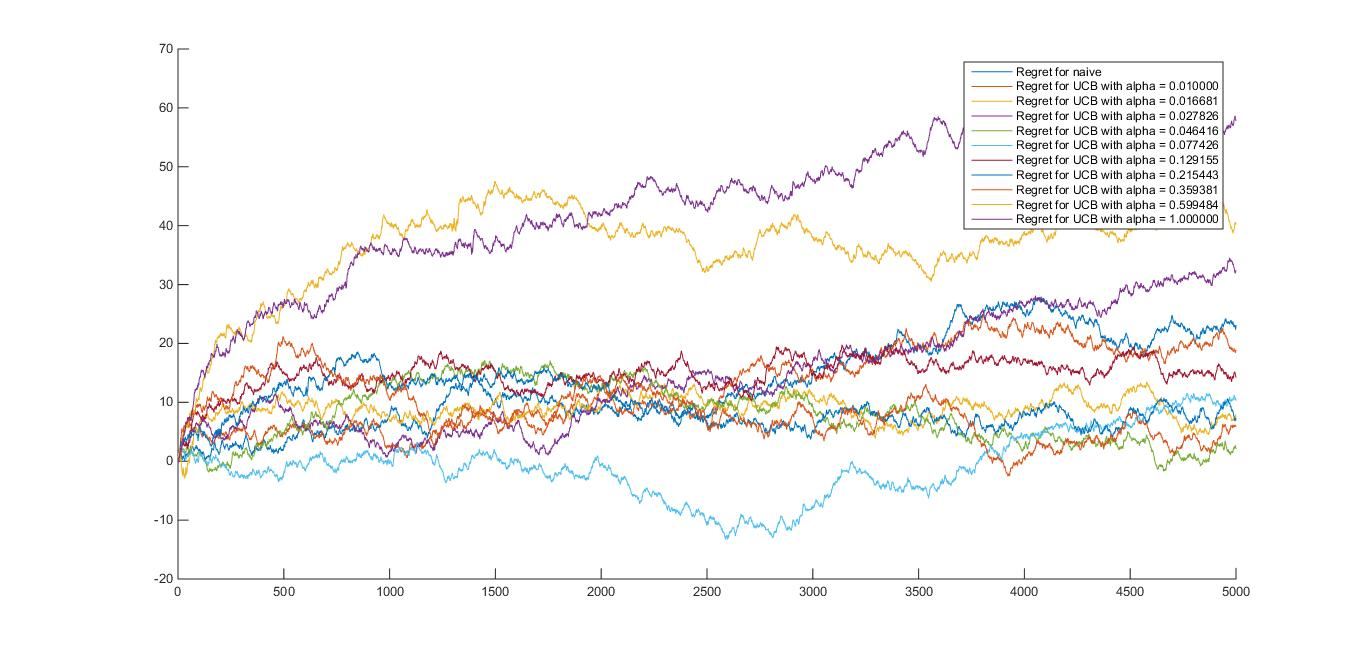
\includegraphics[scale=0.4]{regret_curves.jpg}
	\caption{Regret curves for the naive strategy and the UCB algorithm for several values of $\alpha$}
\end{figure}

\section{Complexity of a bandit problem}

We take a new MAB only composed of Bernoulli arms :
\begin{verbatim}
Arm5 = armBernoulli(0.2);
Arm6 = armBernoulli(0.24);
Arm7 = armBernoulli(0.8);
MAB_easy ={Arm1, Arm7, Arm5, Arm6};
\end{verbatim}

For this MAB, we find as value for the complexity $c = 2,54$, which is low as the maximum mean is distant from the others.

We plot the lower bound and the regret curve :
\begin{figure}[H]
	\centering
	\noindent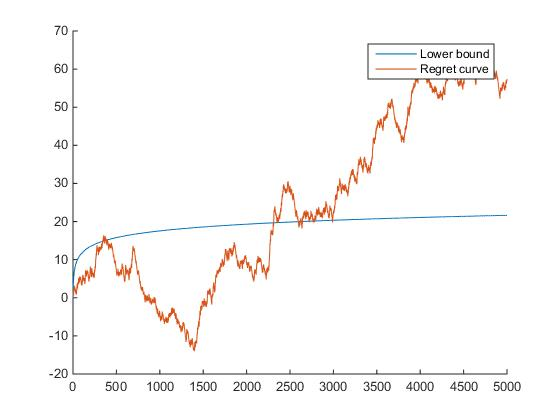
\includegraphics[scale=0.4]{complexity.jpg}
	\caption{Lower bound and regret curve}
\end{figure}

Here, we find effectively that the regret curve is above the lower bound. It might not be the case for another draw, as the result is asymptotic. Here, we stopped at n = 5000.

\section{A Bayesian idea for Bernoulli bandit problems}

"Optimism" consists in letting the agent play as if the environment was the most favorable among all environments that are still sufficiently likely given the observations accumulated so far.

The UCB algorithm is optimistic as because we pull the arm that has the greatest value that is statistically plausible at time t.

Thompson sampling samples each action according to the probability it is optimal. So we cannot say this is an "optimistic algorithm".

\underline{Question 2 :} For the "easy" bandit problem with Bernoulli arms (the same as in section 2), here is what we find :

\begin{figure}[H]
	\centering
	\noindent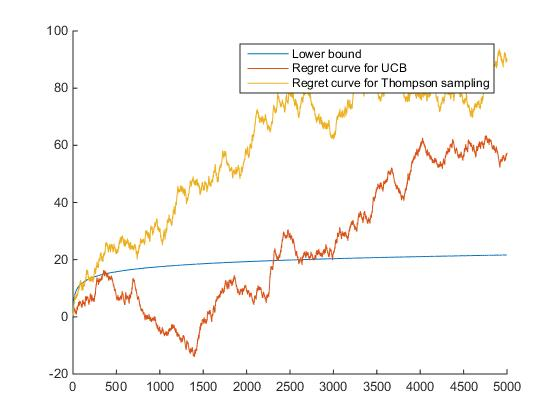
\includegraphics[scale=0.4]{regret_thom_easy.jpg}
	\caption{Lower bound and regret curves for UCB algorithm and Thompson sampling, for an "easy" problem}
\end{figure}

We then implemented this for a more "difficult"proble, as the spread between the means is smaller :
\begin{verbatim}
ArmDiff1 = armBernoulli(0.22);
ArmDiff2 = armBernoulli(0.24);
ArmDiff3 = armBernoulli(0.23);
ArmDiff4 = armBernoulli(0.25);
MAB_diff ={ArmDiff1, ArmDiff2, ArmDiff3, ArmDiff4};
\end{verbatim}

We now have a complexity much larger : $c = 67.7$.
Below is the plot we obtained :
\begin{figure}[H]
	\centering
	\noindent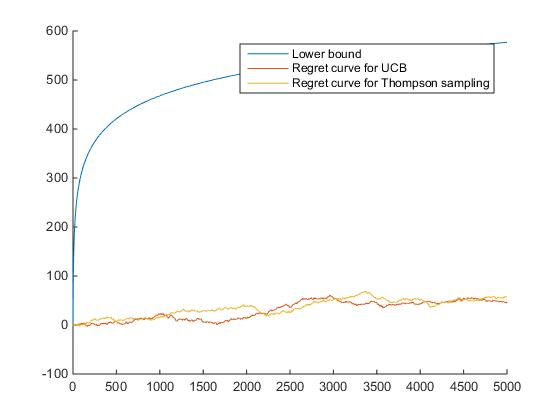
\includegraphics[scale=0.4]{regret_thom_diff.jpg}
	\caption{Lower bound and regret curves for UCB algorithm and Thompson sampling, for a "difficult" problem}
\end{figure}

We immediately see that the horizon is not large enough to have the asymptotic result for the lower bound. For an horizon of 200000 pulls of arms, we got :


\begin{figure}[H]
	\centering
	\noindent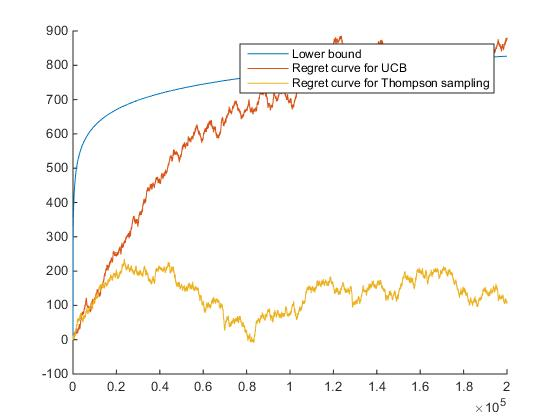
\includegraphics[scale=0.4]{regret_thom_diff2.jpg}
	\caption{Lower bound and regret curves for UCB algorithm and Thompson sampling, for a "difficult" problem}
\end{figure}

On this example we have the lower bound.


\end{document}